\let\negmedspace\undefined
\let\negthickspace\undefined
\documentclass{article}
\usepackage{cite}
\usepackage{amsmath,amssymb,amsfonts,amsthm}
\usepackage{algorithmic}
\usepackage{graphicx}
\usepackage{textcomp}
\usepackage{xcolor}
\usepackage{txfonts}
\usepackage{listings}
\usepackage{enumitem}
\usepackage{tfrupee}
\usepackage{mathtools}
\usepackage{gensymb}
\usepackage[breaklinks=true]{hyperref}
\usepackage{tkz-euclide} % loads  TikZ and tkz-base
\usepackage{listings}
\usepackage{gvv}
%
%\usepackage{setspace}
%\usepackage{gensymb}
%\doublespacing
%\singlespacing

%\usepackage{graphicx}
%\usepackage{amssymb}
%\usepackage{relsize}
%\usepackage[cmex10]{amsmath}
%\usepackage{amsthm}
%\interdisplaylinepenalty=2500
%\savesymbol{iint}
%\usepackage{txfonts}
%\restoresymbol{TXF}{iint}
%\usepackage{wasysym}
%\usepackage{amsthm}
%\usepackage{iithtlc}
%\usepackage{mathrsfs}
%\usepackage{txfonts}
%\usepackage{stfloats}
%\usepackage{bm}
%\usepackage{cite}
%\usepackage{cases}
%\usepackage{subfig}
%\usepackage{xtab}
%\usepackage{longtable}
%\usepackage{multirow}
%\usepackage{algorithm}
%\usepackage{algpseudocode}
%\usepackage{enumitem}
%\usepackage{mathtools}
%\usepackage{tikz}
%\usepackage{circuitikz}
%\usepackage{verbatim}
%\usepackage{tfrupee}
%\usepackage{stmaryrd}
%\usetkzobj{all}
%    \usepackage{color}                                   >
%    \usepackage{array}                                   >
%    \usepackage{longtable}                               >
%    \usepackage{calc}                                    >
%    \usepackage{multirow}                                >
%    \usepackage{hhline}                                  >
%    \usepackage{ifthen}                                  >
  %optionally (for landscape tables embedded in another do>
%    \usepackage{lscape}
%\usepackage{multicol}
%\usepackage{chngcntr}
%\usepackage{enumerate}

%\usepackage{wasysym}
%\documentclass[conference]{IEEEtran}
%\IEEEoverridecommandlockouts
% The preceding line is only needed to identify funding in>

\newtheorem{theorem}{Theorem}[section]
\newtheorem{problem}{Problem}
\newtheorem{proposition}{Proposition}[section]
\newtheorem{lemma}{Lemma}[section]
\newtheorem{corollary}[theorem]{Corollary}
\newtheorem{example}{Example}[section]
\newtheorem{definition}[problem]{Definition}
%\newtheorem{thm}{Theorem}[section]
%\newtheorem{defn}[thm]{Definition}
%\newtheorem{algorithm}{Algorithm}[section]
%\newtheorem{cor}{Corollary}
\newcommand{\BEQA}{\begin{eqnarray}}
\newcommand{\EEQA}{\end{eqnarray}}
%\newcommand{\define}{\stackrel{\triangle}{=}}
\theoremstyle{remark}
\newtheorem{rem}{Remark}

%\bibliographystyle{ieeetr}
\begin{document}
\title{Latex Assignment1}                            \author{APARNA ANAND}
\date{30 August,2023}
\maketitle
\section*{Example:-1-13 (11.12)}
\begin{enumerate}
\item In \figref{fig:12.3}, if $P$ is $(2,4,5)$, find the coordinates of $F$.
\begin{figure}[h]
\centering
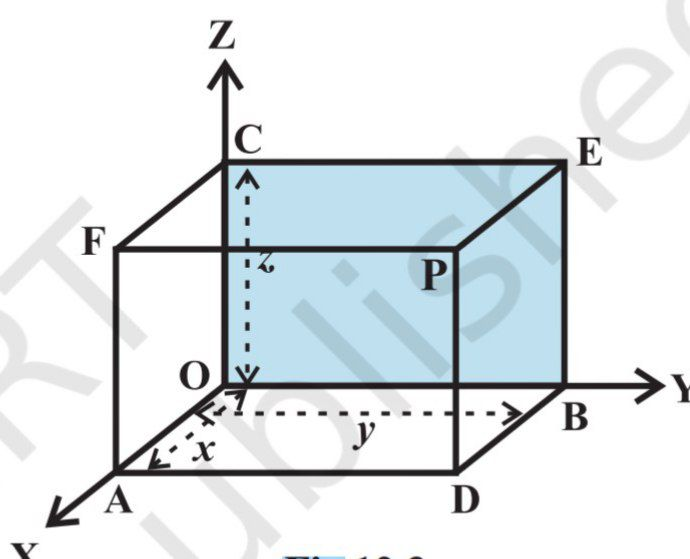
\includegraphics[width=\columnwidth]{figs/12.3.png}
\caption{12.3}
\label{fig:12.3}
\end{figure}
\item Find the octant in which the points $(-3,1,2)$ and $(-3,1,-2)$ lie.
\item Find the distance between the origin $O$ and any point $Q(x_2,y_2,z_2)$.
\item Show that the points $P(-2,3,5), Q(1,2,3)$ and $R(7,0,-1)$ are collinear. 
\item Are the points $A(3,6,9), B(10,20,30)$ and $C(24,-41,5)$ the vertices of a right angled triangle?
\item Find the equation of set of points $P$ such that $PA^2+PB^2=2k^2$, where $A$ and $B$ are the points $(3,4,5)$ and $(-1,3,-7)$, respectively.
\item Find the coordinates of the point which divides the line segment joining the points $(1,-2,3)$ and $(3,4,-5)$ in the ratio $2:3$
\begin{enumerate}[label=(\roman*)]
\item internally, and
\item externally
\end{enumerate}
\item Using section formula, prove that the three points $(-4,6,10), (2,4,6)$ and $(14,0,-2)$ are collinear.
\item Find the coordinates of the centroid of the triangle whose vertices are $(x_1,y_1,z_1), (x_2,y_2,z_2)$ and $(x_3,y_3,z_3)$.
\item Find the ratio in which the line segment joining the points $(4,8,10)$ and $(6,10,-8)$ is divided by the $YZ$- plane.
\item Show that the points $A(1,2,3), B(-1,-2,-1), C(2,3,2)$ and $D(4,7,6)$ are the vertices of a parallelogram $ABCD$, but it is not a rectangle.
\item Find the equation of the set of the points $P$ such that its distances from the points $A(3,4,-5)$ and $B(-2,1,4)$ are equal.
\item The centroid of a triangle $ABC$ is at the point $(1,1,1)$. If the coordinates of $A$ and $B$ are $(3,-5,7)$ and $(-1,7,-6)$, respectively find the coordinates of the point $C$.
\end{enumerate}
\end{document}

